% Created 2018-09-26 Wed 21:07
% Intended LaTeX compiler: pdflatex
\documentclass[journal=ancac3,manuscript=article,email=true,hyperref=true,keywords=false]{achemso}
\usepackage[utf8]{inputenc}
\usepackage{graphicx}
\usepackage{float}
\usepackage{xcolor}
\usepackage{amsmath}
\usepackage{amssymb}
\usepackage{lineno}
\usepackage{todonotes}
\usepackage{times}

\usepackage{xr}
\externaldocument[SI-]{SI}

\author{Tian Tian}
\affiliation{Institute for Chemical and Bioengineering, ETH Z{\"{u}}rich,  Vladimir Prelog Weg 1, CH-8093 Z{\"{u}}rich, Switzerland}
\altaffiliation{T. T. and D. S. contributed equally to this work}
\author{Declan Scullion}
\affiliation{School of Mathematics and Physics, Queen's University Belfast, BT7 1NN, United Kingdom}
\altaffiliation{T. T. and D. S. contributed equally to this work}
\author{Dale Hughes}
\affiliation{School of Mathematics and Physics, Queen's University Belfast, BT7 1NN, United Kingdom}
\author{Lu Hua Li}
\affiliation{Institute for Frontier Materials, Deakin University, Waurn Ponds, Victoria, Australia}
\author{Chih-Jen Shih}
\affiliation{Institute for Chemical and Bioengineering, ETH Z{\"{u}}rich,  Vladimir Prelog Weg 1, CH-8093 Z{\"{u}}rich, Switzerland}
\author{Jonathan Coleman}
\affiliation{School of Physics, Centre for Research on Adaptive Nanostructures and Nanodevices (CRANN) and Advanced Materials and BioEngineering Research (AMBER), Trinity College Dublin, Dublin 2, Ireland.}
\author{Manish Chhowalla}
% \affiliation{Materials Science and Engineering, Rutgers University, 607 Taylor Road, Piscataway, New Jersey 08854, USA.}
\affiliation{Department of Materials Science \& Metallurgy, University of Cambridge, CB3 0FS, United Kingdom}
\author{Elton J. G. Santos}
\email{e.santos@qub.ac.uk}
\affiliation{School of Mathematics and Physics, Queen's University Belfast, BT7 1NN, United Kingdom}
\date{}
\title{The Unified Nature of the Dielectric Properties of Two-Dimensional Materials}
% \title{Unified Understanding of the Dielectric Nature of Two-Dimensional Materials}
\begin{document}

\newpage{}


% \section{Introduction}
% \label{sec:org2ea169d}
\linenumbers{}

{\bfseries Dielectric constant, which defines the polarization of the
  media, is a key quantity in condensed matter. Here we show that
  despite its fundamental transcendence, the dielectric constant does
  not define unequivocally the dielectric properties of a
  two-dimensional (2D) material. We found instead that the dielectric
  polarizability correctly captures the dielectric nature of a 2D
  material which is strongly dependent on the long-range
  electron-electron interaction.  We reveal a long-sought universal
  framework where electronic, geometrical and dielectric properties
  are intrinsically correlated through the polarizability opening the
  door to probe quantities yet not directly measurable, e.g. thickness
  of an atom.  By using this framework, we unify the concept of
  dielectric properties in any material dimension through a dielectric
  anisotropy index which defines the degree of controllability of the
  dielectric features of a compound. A universal boundary line
  separates the 3D and 2D behaviors where materials likely to have
  similar properties as layered materials collapsed onto.  }

The central place of dielectric properties, especially the static
dielectric constant in material research
\cite{Dressel_2001_electrodynamics} drives the pursuit for a unified
model between the electronic and dielectric properties of materials.
% In fact, some pioneering work\cite{Moss_1950_relation} discovered
% relations between the dielectric constant $\varepsilon$ and other
% physical properties, in particular the band gap $E_{\mathrm{g}}$ of
% bulk semiconductors.
In fact, some pioneer
work\cite{Moss_1950_relation,Moss_1985_n_Eg,Ravindra_1979_eps_Eg,Ravindra_2007_Eg_rev}
proposed the empirical model between the energy bandgap
$E_{\mathrm{g}}$ and dielectric constant $\varepsilon$ of bulk
semiconductors, such as the famous Moss relation
\cite{Moss_1950_relation,Moss_1985_n_Eg}:
\begin{equation}
\label{eq:Moss-relations}
\varepsilon^{2} E_{\mathrm{g}} \approx 95\ \mathrm{eV}
\end{equation}
Despite the minor difference between the empirical formulae proposed,
such general relation  is of high
practical importance for material design and engineering: with the
Moss relationship or other similar models, it is feasible to predict
the dielectric constant (and hence other parameters such as refractive
index, Bohr radius, exciton binding energy, etc.) of a bulk material
from the its bandgap with a reasonable degree of certainty
% The
% existence of such general relationship is also of high practical
% importance: it is generally more straightforward and accurate to
% measure the band gap $E_{\mathrm{g}}$ than the static dielectric
% constant $\varepsilon$ of a bulk material, as the latter is strongly
% dependent on several critical details on the sample measurements, such
% as contamination, disorder, and model interpretation.
While the electronic-dielectric relation for bulk semiconductors is
well-established, it is unknown if such equation still exists in
atomically-thin two-dimensional (2D) materials \cite{Novoselov_2016},
due to (i) the dielectric screening of a 2D material is attenuated and
anisotropic
\cite{Keldysh_1979_eps_multi,Sharma_1985,Low_2014_screening_BP,Cudazzo_2011_screening_2D,Bechstedt_2012}
and (ii) the static dielectric constant, a quantity associated with
the macroscopic dielectric and optoelectronic properties and commonly
obtained by theoretical calculations of 2D materials
\cite{Ramasubramaniam_2012,Wang_2016_Aip,Laturia_2018}, may not well
describe this microscopic and anisotropic dielectric nature of 2D
materials \cite{Cudazzo_2010_screen2D,Cudazzo_2011_screening_2D}.
% Therefore, an
% accurate description of the 2D dielectric nature is the prerequisite
% for a 2D Moss-like relation, which could be used to make predictions
% for less-investigated layered crystals and to create materials design
% rules at an accurate level.
Here we show that instead of the dielectric constant,
the 2D polarizabilty correctly captures the dielectric nature
of a 2D material. Based on both theoretical model and first principle
calculations, we reveal the long-sought universal dielectric scaling
relations for 2D materials, depend both on the electronic and
structural information: the in-plane polarizability
$\alpha^{\parallel}_{\mathrm{2D}}$ is inversely proportional to the minimal bandgap
$E_{\mathrm{g}}$, while the out-of-plane polarizability
$\alpha^{\perp}_{\mathrm{2D}}$ is directly related with the thickness
$\delta$ of a 2D materials. We further introduce the concept of
dielectric anisotropy index, to unify 2D and 3D dielectric
property. The proposed universal dielectric scaling relationships of
2D compounds introduce a general pathway for the exploration of their
complex physical and chemical phenomena well beyond the currently
possible applications.
% Based on this
% framework, we further unify the concept of dielectric properties of
% any material dimension, by the dielectric anisotropy index, 
% An analytical quantum-mechanical model is developed
% which give a sound background to the dielectric-scale
% relationships.
% Using such unified relations unify the dielectric
% properties between the 2D materials and their 3D counterparts in a
% natural manner, which ultimately pushes the boundary of the
% understanding of electronic screening in both dimensions.
% The discovery of scaling relationships between dielectric and electronic
% and structural properties in 2D compounds introduces a new and general
% pathway for the exploration of their complex physical and chemical
% phenomena well beyond the currently possible applications.

% \section{Results}
% \label{sec:org752ca78}

\subsection{Dielectric Nature of 2D Materials}
\label{sec:2d}

In pursuit of the Moss-like relation for 2D materials, an accurate
description of their dielectric properties needs to be established,
since the concept of macroscopic dielectric constant is ill-defined
for 2D materials
\cite{Cudazzo_2010_screen2D,Cudazzo_2011_screening_2D,Nazarov_2015_2D_3D}. As
shown in Figure \ref{fig-1}a, in routine first principles
calculations, an isolated 2D material is placed in the xy-plane of a
periodically repeating superlattice (SL) with a length $L$ along the
z-direction separating the cell images. The macroscopic dielectric
tensor from the superlattice $\varepsilon_{\mathrm{SL}}^{pq}$, is
determined through fundamental electrostatics by the response of the
polarization density $\boldsymbol{P}^{p}$ under small perturbative
external field $\boldsymbol{E}^{q}$, where $p$, $q$ are the directions
of polarization and electric field,
respectively\cite{Dressel_2001_electrodynamics}:
\begin{subequations}
  \begin{eqnarray}
      \label{eq:def-eps-1}
    &\varepsilon^{pq} &= \kappa^{pq} +
                                 {\displaystyle \frac{\partial \boldsymbol{P}^{p}}
                                 {\varepsilon_{0} \partial \boldsymbol{E}^{q}}} \\
          \label{eq:def-eps-2}
    &\boldsymbol{P}^{p} &=  {\displaystyle \frac{\boldsymbol{u}^{p}}{\Omega}}
                          = {\displaystyle \frac{{\displaystyle
          \int_{\mathrm{SL}} \rho(\boldsymbol{r}) \boldsymbol{r}^{p} d^{3}\boldsymbol{r}}}
                          {AL}}
  \end{eqnarray}
\end{subequations}
where $\kappa$ is the dielectric tensor of the environment,
$\boldsymbol{u}$ is the total dipole moments within the SL, $\rho$ is the
spatial charge density, $\Omega=AL$ is the volume, $A$ is the xy-plane
area of the SL and $\varepsilon_{0}$ is vacuum permittivity. For the
majority of 2D semiconductors, the off-diagonal elements of the
dielectric tensor ($p \neq q$) tend to be negligible.  Considering
that the 2D material is placed in vacuum ($\kappa^{pp} = 1$ and
$\kappa^{pq} = 0$), we can distinguish two components, namely the
in-plane ($\varepsilon_{\mathrm{SL}}^{\parallel}$) and out-of-plane
($\varepsilon_{\mathrm{SL}}^{\perp}$) dielectric constants, where
$\varepsilon_{\mathrm{SL}}^{\parallel} =
(\varepsilon_{\mathrm{SL}}^{xx} + \varepsilon_{\mathrm{SL}}^{yy})/2$
and
$\varepsilon_{\mathrm{SL}}^{\perp} =
\varepsilon_{\mathrm{SL}}^{zz}$. The absence of bonding perpendicular
to the 2D plane confines the induced dipoles along the
\textit{z}-direction: as shown in Figure \ref{fig-1}a and
Supplementary Figure \ref{SI-fig:rho-profile}, the charge density difference
between zero and finite electric fields,
$\Delta \rho=\rho(\boldsymbol{E}) - \rho(\boldsymbol{E}=0)$ along the
z-axis for an isolated 2H-MoS$_{2}$ layer under
$|\boldsymbol{E}_{z}|=0.01 \mathrm{V\cdot \AA}^{-1}$ only extends to
$\sim{}$12 \AA{} along the z-direction. When $L$ is large enough that
the induced dipoles from periodic images do not interact,
$\boldsymbol{u}$ equals the total dipole moments of a monolayer 2D
materials and independent of the SL size. As a consequence, we can see
from Eqs. \ref{eq:def-eps-1} and \ref{eq:def-eps-2}, that both
$\varepsilon^{\parallel}_{\mathrm{SL}}$ and
$\varepsilon^{\perp}_{\mathrm{SL}}$ depend on $L$. We show this by
plotting $\varepsilon^{\parallel}_{\mathrm{SL}}$ and
$\varepsilon^{\perp}_{\mathrm{SL}}$ calculated from density functional
theory (DFT) as functions of $L$ for P$\bar{6}$m2 (2H) transitional
metal dichalcogenides (TMDCs, 2H-MX$_{2}$, where M=Mo, W and X=S, Se,
Te), in the top panels of Figure \ref{fig-1}b and \ref{fig-1}c,
respectively.
% We observe that neither
% $\varepsilon^{\parallel}_{\mathrm{SL}}$ nor
% $\varepsilon^{\perp}_{\mathrm{SL}}$ converges with $L$ due to fact
% that the long-range Coulomb interaction could not be completed
% screened within the range of magnitudes computationally accessible
% \cite{Hueser_2013_2Dvs3D}.
As a result, the $L$-dependency of $\varepsilon_{\mathrm{SL}}$ makes
it impractical to represent the dielectric nature of a 2D material
both theoretically and experimentally, because the size of vacuum
layer must always be considered. To solve this problem, we need to
find the $L$-independent alternative of
$\varepsilon_{\mathrm{SL}}$. As described before, by multiplying
Eq. \ref{eq:def-eps-2} with $L$ we get the sheet polarization density
of a 2D material $\boldsymbol{\mu}_{\mathrm{2D}}$, such that
$\boldsymbol{\mu}_{\mathrm{2D}}^{p} = \boldsymbol{P}^{p}L =
\boldsymbol{u}^{p}/A$, which is dependent with $L$ due to the invariablity
of $\boldsymbol{u}$ and $A$. Similar to the definition of molecular
polarizability \cite{Israelachvili_2011},
$\boldsymbol{\mu}_{\mathrm{2D}}$ is associated with the 2D
polarizability $\alpha_{\mathrm{2D}}$ through:
$\boldsymbol{\mu}^{p} = \sum_{q} \alpha_{\mathrm{2D}}^{pq}
\boldsymbol{E}_{\mathrm{loc}}^{q}$ \cite{T_bik_2004}, where
$\boldsymbol{E}_{\mathrm{loc}}$ is the local electric field. In the
in-plane direction, the continuity of electric field gives
$\boldsymbol{E}^{\parallel}_{\mathrm{loc}}=\boldsymbol{E}^{\parallel}$
\cite{Markel_2016}. Perpendicular to the 2D plane, the dipole
screening yields
$\boldsymbol{E}_{\mathrm{loc}}^{\perp}=\boldsymbol{E}^{\perp}+\boldsymbol{\mu}_{\mathrm{2D}}^{\perp}/L$
\cite{Meyer_2001_dipole_slab,T_bik_2004}. Combining with
Eqs. \ref{eq:def-eps-1} and \ref{eq:def-eps-2}, we can relate the 2D polarizabilities,
$\alpha_{\mathrm{2D}}^{\parallel}$ and $\alpha_{\mathrm{2D}}^{\perp}$ with $\varepsilon_{\mathrm{SL}}^{\parallel}$ and $\varepsilon_{\mathrm{SL}}^{\perp}$, respectively:
% \begin{subequations}
% \begin{eqnarray}
  % \label{eq:alpha-para-def}
  % &\alpha_{\mathrm{2D}}^{\parallel} &= \varepsilon_{0}(\varepsilon_{\mathrm{SL}}^{\parallel} - 1)L\\
  % \label{eq:alpha-perp-def}
  % &\alpha_{\mathrm{2D}}^{\perp} &= \varepsilon_{0}\left(1 - {\displaystyle \frac{1}{\varepsilon_{\mathrm{SL}}^{\perp}}}\right)L
% \end{eqnarray}
% \end{subequations}
\begin{subequations}
\begin{eqnarray}
  \label{eq:alpha-para-def}
  &\varepsilon_{\mathrm{SL}}^{\parallel} &= 1 + \frac{\alpha_{\mathrm{2D}}^{\parallel}}{\varepsilon_{0}L}\\
  \label{eq:alpha-perp-def}
  &\varepsilon_{\mathrm{SL}}^{\perp} &= \left(1 - {\displaystyle \frac{\alpha_{\mathrm{2D}}^{\perp}}{\varepsilon_{\mathrm{0}} L}} \right)^{-1}
\end{eqnarray}
\end{subequations}
The bottom panels of Figure \ref{fig-1}b and \ref{fig-1}c show the
$\alpha_{\mathrm{2D}}^{\parallel}$ and $\alpha_{\mathrm{2D}}^{\perp}$
of the TMDCs as functions of $L$, calculated using
Eqs. \ref{eq:alpha-para-def} and \ref{eq:alpha-perp-def}. We observe
that both $\alpha_{\mathrm{2D}}^{\parallel}$ and
$\alpha_{\mathrm{2D}}^{\perp}$ remain almost constant when $L>$15
\AA{}. In addition, as shown Figure \ref{fig-1}d and \ref{fig-1}e,
respectively, the model-predicted
$\varepsilon_{\mathrm{SL}}^{\parallel}-L$ and
$\varepsilon_{\mathrm{SL}}^{\perp}-L$ relations from Eqs.
\ref{eq:alpha-para-def} and \ref{eq:alpha-perp-def} nicely reproduce
the trends from Figures \ref{fig-1}b and \ref{fig-1}c. These findings
indicate that the 2D polarizability, instead of the dielectric
constant, is the true descriptor of the dielectric properties of 2D
materials. More discussion about the choice of the 2D polarizability
and comparison with other methods can be find in Supplementary Section
\ref{SI-sec:2D-3D-rescale}.


\subsection{2D Moss-like  Relations}
\label{sec:first-principles}
Based on the 2D polarizabilities, we then investigate the potential
Moss-like relations for 2D materials. By evaluating the expressions
for $\alpha_{\mathrm{2D}}^{\parallel}$ and
$\alpha_{\mathrm{2D}}^{\perp}$ using Random Phase Approximation (RPA)
theory \cite{Adler_1962} with $\mathbf{k} \cdot \mathbf{p}$
treatment\cite{kittel_2005_introduction} (details see Supplementary
Section \ref{SI-ssec:theory-1}), we show that
$\alpha_{\mathrm{2D}}^{\parallel}$ and $\alpha_{\mathrm{2D}}^{\perp}$
have simple relation with the electronic  and structural information of a 2D
material, respectively:
\begin{subequations}
\begin{eqnarray}
\label{eq:2D-Moss-para}
  &\alpha_{\mathrm{2D}}^{\parallel} &\propto E_{g}^{-1} \\
  \label{eq:2D-Moss-perp}
  &\alpha_{\mathrm{2D}}^{\perp} & \propto \delta
\end{eqnarray}
\end{subequations}
where $E_{\mathrm{g}}$ is the minimal electronic bandgap of the 2D
material, and $\delta$ is its intrinsic
thickness. Eqs. \ref{eq:2D-Moss-para} and \ref{eq:2D-Moss-perp} are
the main conclusions of this work.  \todo[inline]{I not sure if we
  need to show the proportional coefficients
  here. $\alpha_{2D}^{\perp}$ is almost certain to be
  $\varepsilon_{0}\delta$, but $\alpha_{\mathrm{2D}}^{\parallel}$ has
  a more complex coefficient.}

To validate such relations, we study several types of 2D materials as
show in Figure \ref{fig-3}a, including transition metal
dichalcogenides (TMDCs, with the formula MX\(_{\text{2}}\), where M is
a metal in groups 4, 6, 10 and X=O, S, Se, Te), metal monochalcogenides
(Ga$_{2}$S$_{2}$, Ga$_{2}$Se$_{2}$), cadmium halides (CdX$_2$, X=Cl,
I), hexagonal boron nitride (BN), graphene derivatives (fluorographene
(C$_{2}$F$_{2}$), graphane (C$_{2}$H$_{2}$)), phosphorene (P$_{4}$)
and thin layer organic-inorganic perovskites (ABX$_{3}$).  For the
TMDCs, we consider 2 lattice phases, namely the 2H (P\(\bar{6}\)m2
space group) and 1T (P3m1 space group).  The static 2D
polarizabilities are calculated from the static dielectric response of
the selected 2D materials using density functional theory (DFT) with
the Heyd-Scuseria-Ernzerhof hybrid functionals (HSE06) using the
Vienna Ab Initio Simulation Package (VASP) including spin-orbit
coupling to avoid limitations on the description of band gaps and
dielectric functions (see Methods for details). Figure \ref{fig-3}b
shows the calculated $E_{\mathrm{g}}$ (blue dots) and polarizabilities
(bar plots) of all the 2D materials investigated, covering a wide
spectrum range from far infrared to ultraviolet. Note from dimension
analysis, it is more intuitive to express the polarizability as
$\alpha_{\mathrm{2D}}/(4 \pi \varepsilon_{0})$, which has unit of
\AA. We find that $\alpha_{\mathrm{2D}}^{\parallel}$ has a general
descending trend when $E_{\mathrm{g}}$ increases. On the other hand,
no apparent correlation between $\alpha_{\mathrm{2D}}^{\perp}$ and
$E_{\mathrm{g}}$ is observed (see Supplementary Section
\ref{SI-sec:pol-2D-Eg}), which appears to be in good agreement with
our polarizability-based theoretical model (Supplementary Section
\ref{SI-ssec:theory-2}). We then examine Eqs. \ref{eq:2D-Moss-para}
and \ref{eq:2D-Moss-perp} using the polarizabilities calculated by
first principle calculations. Figure \ref{fig-3}b shows
$(4 \pi \varepsilon_{0})/\alpha_{\mathrm{2D}}^{\parallel}$ (in
\AA{}$^{-1}$) as a function of $E_{\mathrm{g}}$ (in eV) for the 2D
materials investigated (circle dots), with a linear regression
coefficient of regression $R^{2}$ of 0.84, and a slope of 0.18, which
corresponds well with theoretical investigations (details see
Supplementary Section \ref{SI-sssec:theory-1}).  We also discover that
the linearity between
$(4 \pi \varepsilon_{0})/\alpha_{\mathrm{2D}}^{\parallel}$ and
$E_{\mathrm{g}}$ (measured by the $R^{2}$ value) is higher when the
bandgap is calculated using the HSE06 hybrid functionals, compared
with that from the Perdew--Burk--Ernzerhof (PBE) exchange correlations
(details see Supplementary Section \ref{SI-sec:pol-2D-Eg} and
Supplementary Figure \ref{SI-fig:alpha-Eg-diff}), which can be
explained by the fact that the electronic structure, in particular the
bandgap, is generally better predicted at HSE06 level than PBE level
\cite{Heyd_2005}. It should be noted that although even more accurate
estimation of both dielectric properties and bandgap can be achieved
via many-body Green's function method (GW) together with the
Bethe-Salpeter equation (BSE), the convergence of such method is known
to be highly affected by the dielectric screening of 2D materials
\cite{Hueser_2013_2Dvs3D}. Combining the accuracy, computational
effort and convergence, the choice of the HSE06 hybrid functional may
be most suitable to present the true 2D Moss-like relationship between
$\alpha_{\mathrm{2D}}^{\parallel}$ and $E_{\mathrm{g}}$. We also show
that the proposed relation behaves equivalently well when using the
experimentally accessible optical bandgap of 2D materials (details see
Supplementary Section \ref{SI-sec:gpaw-2} and Supplementary Figure
\ref{SI-fig:opt}).

We further examine the relation between $\alpha_{\mathrm{2D}}^{\perp}$ and the
thickness of a 2D material proposed in
Eq. \ref{eq:2D-Moss-perp}. Here we choose the ``covalent'' thickness
$\delta_{\mathrm{cov}}$ of a 2D material, which is defined as the
longest distance along the z-direction between any two atom nuclei
plus their covalent radii:
\begin{equation}
  \label{eq:cov-thick}
  \delta_{\mathrm{cov}} = \mathrm{max}(|z^{i} - z^{j}|
  + r^{i}_{\mathrm{cov}} + r^{j}_{\mathrm{cov}})
\end{equation}
where i, j are two atoms in the 2D material and $r_{\mathrm{cov}}^{i}$
is the covalent radius of atom i (Figure \ref{fig-3}c inset). As shown
in Figure \ref{fig-3}c,
$\alpha_{\mathrm{2D}}^{\perp}/(4 \pi \varepsilon_{0})$ indeed shows an
excellent linear correlation with $\delta_{\mathrm{cov}}$, with
$R^{2}=0.98$, and the slope very close to $1/4\pi$. In other words, we
propose
$\alpha_{\mathrm{2D}}^{\perp} / \varepsilon_{0} \approx
\delta_{\mathrm{cov}}$, which has its strong physical meaning. Similar
to the molecular polarizability which characterizes the volume of
electron cloud of an isolated molecule \cite{Israelachvili_2011},
$\alpha_{\mathrm{2D}}^{\perp}/\varepsilon_{0}$ is also related to the
volume of the electron cloud per unit area (from its definition), and
is naturally proportional to the electron cloud thickness of the 2D
material (see Supplementary Section \ref{SI-sssec:theory-3}). In fact,
the universal scaling relation for $\alpha_{\mathrm{2D}}^{\perp}$ in
Figure \ref{fig-3}c indicates that the quantity
$\alpha_{\mathrm{2D}}^{\perp}/\varepsilon_{0}$ measurable via
electronic approaches
\cite{Antoine_1999,Cherniavskaya_2003,Krauss_1999_EFM}, is indeed the
(dielectric) characteristic thickness of a 2D material, and can be
used to resolve the long-existing controversy about the experimental
thickness of 2D materials, such as graphene \cite{Shearer_2016}.

To rule out the possibility that our conclusion is limited by the
number of materials used, we further validate our proposed 2D
Moss-like relations on the recently published C2DB database
\cite{Haastrup_2018}, from which we extracted the dielectric
properties of over 230 2D materials calculated at the PBE level, and
superimpose with our results in Figure \ref{fig-3}b and \ref{fig-3}c
(details see Supplementary Section \ref{SI-sec:gpaw-1}). Although the
dielectric properties may be overestimated at PBE level due to
underestimation of the bandgap compared with the more accurate HSE06
functionals \cite{Van_Dyck_2017}, similar linear trends can be
observed for both $\alpha^{\parallel}_{\mathrm{2D}}$ and
$\alpha_{\mathrm{2D}}^{\perp}$, with the linear coefficient very close
to the HSE06 results (details see Supplementary Section
\ref{SI-sec:gpaw-2}). We have also tested the potential relation
between the 2D polarizabilities with other physical quantities,
including the effective carrier mass, quantum capacitance and total
atomic polarizabilities, while no apparent correlations are found
(details see Supplementary Section \ref{SI-sec:gpaw-3}).

In short, we have revealed the 2D analog of the Moss relation by both
theoretical modeling and first principles calculations:
$\alpha_{\mathrm{2D}}^{\parallel}$ is inversely proportional to the
minimal bandgap $E_{\mathrm{g}}$, while $\alpha_{\mathrm{2D}}^{\perp}$
is the characteristic thickness of the 2D material. Next we show,
despite their different forms, both 2D Moss-like relations stem from
the same origin. In merit of the unit analysis,
$\alpha_{\mathrm{2D}}^{\parallel}$ and $\alpha_{\mathrm{2D}}^{\perp}$
both have unit of $4\pi\varepsilon_{0} \cdot$[Length], or in other
words, $\alpha_{\mathrm{2D}}^{\parallel}$ and
$\alpha_{\mathrm{2D}}^{\perp}$ correspond to in- and out-of-plane
characteristic lengths, respectively. The in-plane screened
electrostatic potential $V(r)$ from a point charge in an 2D plane, as
a function of distance $r$:
$V(r) = {\displaystyle \frac{e}{4 \alpha_{\mathrm{2D}}^{\parallel}}}
\left[H_{0}({\displaystyle \frac{2\varepsilon_{0}
      r}{\alpha_{\mathrm{2D}}^{\parallel}}}) - Y_{0}( {\displaystyle
    \frac{2
      \varepsilon_{0}r}{\alpha_{\mathrm{2D}}^{\parallel}}})\right]$
\cite{Keldysh_1979_eps_multi,Pulci_2014}, where $H_{0}$ is the Struve
function and $Y_{0}$ is the Bessel function of second kind, is
associated with the in-plane screening radius
$r_{0}^{\parallel}=\alpha_{\mathrm{2D}}^{\parallel}/(2
\varepsilon_{0})$, such that $V(r,r/r^{\parallel}_{0} \gg 1)$ reduces
to the simple Coulomb potential in vacuum. Combining with the result
that $\alpha_{\mathrm{2D}}^{\perp}/\varepsilon_{0}$ characterizes the
thickness of a 2D material, we have drawn a generalized picture of the
dielectric nature of 2D materials via the 2D polarizability: the
dielectric screening of a point charge sitting in the middle of a 2D
material can be viewed as an ellipsoid with the length of principle
axes to be
$r_{0}^{\parallel} = \alpha_{\mathrm{2D}}^{\parallel}/(2
\varepsilon_{0})$ and
$r_{0}^{\perp} = \alpha^{\perp}_{\mathrm{2D}}/(2 \varepsilon_{0})$,
respectively, analog to the polarizability ellipsoid picture of
molecules used in spectroscopy \cite{Banwell_1994} (see Supplementary
Figure \ref{SI-fig:ellipsoid}). The polarizability ellipsoid for a 2D
material is in general ultra flat, with
$r_{0}^{\parallel} \gg r_{0}^{\perp}$, as can be seen from the group 6
TMDCs in Table \ref{tbl:radii}\todo{Lacks MoSe2}.  Moreover,
$r_{0}^{\parallel}$ is generally larger for a smaller bandgap
semiconductor, which qualitatively explains the inverse proportional
relation between $\alpha_{\mathrm{2D}}^{\parallel}$ and
$E_{\mathrm{g}}$, a 2D version of the Moss-relation.


\subsection{Bridging the 2D and 3D Dielectric Properties}
\label{sec:2D-3D}

The universal Moss-like relation shown in the previous sections
provides general understanding of the dielectric nature of 2D
materials. Moreover, the underlying physical mechanism allows us to
further bridge the 2D and 3D dielectric and electronic properties in
various ways. Using the similar approach as we derive the 2D Moss-like
relations, we show that the
$\alpha_{\mathrm{2D}}^{\parallel} \propto E_{\mathrm{g}}^{-1}$
relation for a 2D material naturally transforms to
$\varepsilon \propto E_{\mathrm{g}}^{-\frac{1}{2}}$ for a bulk
semiconductor, which is the original Moss relation (details see
Supplementary Section \ref{SI-ssec:theory-2}). In other words, the
proposed $\alpha_{\mathrm{2D}}^{\parallel}-E_{\mathrm{g}}$ relation is
indeed the Moss relation in 2D world, while the different power law
for $E_{\mathrm{g}}$ is caused by the electronic confinement.
\todo[inline]{I shortened this paragraph since the derivation is
  interesting but not so much related with other stuff like the
  dielectric anisotropy.}

The dielectric constant $\varepsilon$, although not well-defined for
monolayer 2D material, becomes applicable when the 2D layers are
stacked. \todo[inline]{I would appreciate for polishing this sentence}
In a bulk layered material stacked by layers with equilibrium
inter-layer distance $L_{\mathrm{Bulk}}$, we define the polarizability
of individual layer $\alpha_{\mathrm{2D}}(L=L_{\mathrm{Bulk}})$ as
$\alpha_{\mathrm{Bulk}}$. Inspired by Eqs. \ref{eq:alpha-para-def} and
\ref{eq:alpha-perp-def}, the dielectric constants
$\varepsilon^{\parallel}_{\mathrm{Bulk}}$ and
$\varepsilon^{\perp}_{\mathrm{Bulk}}$ of a bulk layered material, can
be reconstructed by $\alpha_{\mathrm{Bulk}}^{\parallel}$ and
$\alpha_{\mathrm{Bulk}}^{\perp}$ (see Figure \ref{fig-4}a):
\begin{subequations}
\begin{align}
  \label{eq:3D-para}
  \varepsilon^{\parallel}_{\mathrm{Bulk}}
  &= 1 + \frac{\alpha_{\mathrm{bulk}}^{\parallel}}{\varepsilon_{0} L_{\mathrm{Bulk}}}
  \approx 1 + \frac{\alpha_{\mathrm{2D}}^{\parallel}}{\varepsilon_{0} L_{\mathrm{Bulk}}} \\
  \label{eq:3D-perp}
  \varepsilon^{\perp}_{\mathrm{Bulk}}
  &= \left(1 - \frac{\alpha_{\mathrm{Bulk}}^{\perp}}{\varepsilon_{0} L_{\mathrm{Bulk}}}\right)^{-1}
  \approx \left(1 - \frac{\alpha_{\mathrm{2D}}^{\perp}}{\varepsilon_{0} L_{\mathrm{Bulk}}}\right)^{-1}
\end{align}
\end{subequations}
The approximations come from the fact that
$\alpha_{\mathrm{Bulk}} \approx \alpha_{\mathrm{2D}}$, which can be
seen from the results of Figure \ref{fig-3}b and \ref{fig-3}c.  Note
that the effect of stacking is not considered in Eqs. \ref{eq:3D-para}
and \ref{eq:3D-perp}. We compare the values of
$\varepsilon_{\mathrm{bulk}}^{\parallel}$ and
$\varepsilon_{\mathrm{bulk}}^{\perp}$ from DFT calculations (y-axis)
with those predicted using Eqs \ref{eq:3D-para} and \ref{eq:3D-perp}
(x-axis), as show in Figure \ref{fig-4}b and \ref{fig-4}c,
respectively, with data calculated at both HSE06 and PBE levels give
almost identical trends. We observe that
$\varepsilon_{\mathrm{bulk}}^{\parallel}$ values calculated by DFT and
predicted by Eq. \ref{eq:3D-para} are in good agreement, with a linear
regression slope of 1.01 and $R^2$ of 0.97. On the other hand,
$\varepsilon_{\mathrm{bulk}}^{\perp}$ values predicted from
Eq. \ref{eq:3D-perp} agree well with the DFT-calculated values when
$E_{\mathrm{g}}>4$ eV, while the deviation becomes larger when
$E_{\mathrm{g}}$ reduces. The above results indicate that
$\alpha^{\parallel}_{\mathrm{Bulk}}$ can generally be estimated from
its 2D counterpart, while $\alpha^{\perp}_{\mathrm{Bulk}}$ differs due
to interlayer coupling and overlap between induced
dipoles\cite{Andersen_2015_dielec_vdWH,Laturia_2018}, as also observed
in Figure \ref{fig-3}b, \ref{fig-3}c . With a better model describing
$\alpha_{\mathrm{bulk}}^{\perp}$ as function of $\alpha_{\mathrm{2D}}^{\perp}$ and
the degree of interlayer coupling, the dielectric transition from 2D
to 3D would be smoothly described.

Finally, we show that a general picture of the dielectric properties in
both dimensions can be drawn by studying the dielectric
anisotropy. We define the dielectric anisotropy index $\eta$ as:
\begin{equation}
  \label{eq:anisotropy}
  \begin{aligned}[t]
    \eta =
    \begin{cases}
      {\displaystyle \min_{i \neq j}}
      {\displaystyle
        \left(\frac{\varepsilon^{ii}}{\varepsilon^{jj}}\right)},
      \ \mathrm{Bulk\ Materials}\\
      {\displaystyle \min_{i \neq j}}
      {\displaystyle
        \left(\frac{\alpha_{\mathrm{2D}}^{ii}}{\alpha_{\mathrm{2D}}^{jj}}\right)},
      \ \mathrm{2D\ Materials}\\
    \end{cases}
  \end{aligned}
\end{equation}
$\eta=1$ indicates the material has isotropic dielectric properties
while $\eta \to 0$ means the dielectric property is highly
anisotropic. Figure \ref{fig:aniso} shows the phase diagram of $\eta$
as function of $E_{\mathrm{g}}$ for 2D materials and their bulk
counterparts. Interestingly, the 2D materials (blue triangle) can be
clearly distinguished from the bulk layered materials (orange square)
with the boundary line determined to be
$\eta =0.048 (E_{\mathrm{g}}/ \mathrm{eV})+0.087$. The much lower
$\eta$ values for 2D materials compared with their bulk counterparts
indicates a high dielectric anisotropy, which is responsible for the
unique 2D optoelectronic properties, such as electrostatic
transparency \cite{Liluhua_2014,Tian_2016,Li_2018} and large exciton
binding energy
\cite{Pulci_2014,Tran_2014,Chernikov_2014_EB_MoS2_2D3D,Berkelbach_2013}. From
Eqs. \ref{eq:2D-Moss-para}, \ref{eq:2D-Moss-perp} and
\ref{eq:anisotropy} we can see $\eta$ is roughly proportional to
$\delta \cdot E_{\mathrm{g}}$, which explains the observation that
$\eta$ for 2D materials increase almost linearly with
$E_{\mathrm{g}}$, since the layer thickness $\delta$ (mostly 3--10
\AA{}) of the 2D materials investigated varies much less than
$E_{\mathrm{g}}$ (0.1--7 eV) (Figure \ref{fig-3}b and
\ref{fig-3}c). Further analysis shows that the dielectric anisotropy
index of any bulk layered material $\eta_{\mathrm{Bulk}}$ obeys
$\eta_{\mathrm{Bulk}} \geq {\displaystyle \frac{4
    \eta_{\mathrm{2D}}}{(\eta_{\mathrm{2D}}+1)^{2}}} \geq
\eta_{\mathrm{2D}}$, where $\eta_{\mathrm{2D}}$ is the anisotropy
index of corresponding 2D layer (details see Supplementary Section
\ref{SI-sssec:aniso-2}), which is the basis for the separation of bulk
and 2D regimes in the $\eta-E_{\mathrm{g}}$ phase diagram.  For
comparison, we also superimpose the dielectric anisotropy indices
$\eta$ of common semiconducting materials in other dimensions (details
see Supplementary Section \ref{SI-sssec:aniso-1}) on the phase diagram in Figure
\ref{fig:aniso}. Bulk covalent (3D, e.g. Si, GaN) and 0D (fullerenes)
semiconductors show isotropic dielectric properties, scattered on the
line $\eta=1$. On the other hand, reduced dimensionality increases the
dielectric anisotropy of materials such as planar organic
semiconductor (OSc, 1D-2D, e.g. CuPc), carbon nanotube (CNT, 1D),
linear OSc (0D-1D, e.g. polyacene and polyacetylene). Interestingly,
most of these materials also scatter along the boundary line
separating the bulk and 2D regimes, indicating the criteria
distinguishing 2D (more anisotropic) and bulk layered materials (more
isotropic) from the $\eta-E_{\mathrm{g}}$ diagram, can also be applied
to other dimensions. From the phase diagram, we can see that 2D and
bulk layered materials (also including 2D van der Waals
heterostructure (vdWH) \cite{Novoselov_2016}), provides more
flexibility in controlling the dielectric and electronic properties,
compared with semiconductors in other dimensions.  \todo[inline]{I
  leave this section to be freely modified}



\subsection{Implications for Experiments}
\todo[inline]{Wait for comments from JC and MC.}


\section{Conclusion}
\label{sec:org5fd1f1a}
\todo[inline]{To be changed later when everything fixed}
To sum up, using first principles calculation for a large set of 2D
materials, we reveal the universal relation of the dielectric nature
of 2D materials using the 2D polarizability, as an analog to the Moss
relation for bulk semiconductors. The in-plane polarizability of a 2D
material is found to be inversely proportional to the minimal bandgap,
while the out-of-plane polarizability is the characteristic thickness
of the 2D material. Such universal scaling relation is explained by a
quantum mechanical model combining the polarizability in both
directions. Our universal scaling relation bridges the gap between 2D
and 3D dielectric properties with good accuracy of prediction.  Our
numerical findings and theoretical analysis pave the way to understand
and engineer the electronic and dielectric properties of a large
library of 2D materials for different technological applications in an
unified and unprecedented way.

\section{Theoretical Methods}
\label{sec:org8457dbb}

All results calculated for this paper were the result of \emph{ab
  initio} simulations carried out using plane-wave Density Functional
Theory (DFT) package VASP
\cite{Kresse_1993,Kresse_1996_1,Kresse_1996_2} using the Projector
Augmented Wave (PAW) approach with Kresse's mainly GW
Pseudopotentials \cite{Kresse_1999_pseudopotentials}. Band gaps were
calculated using the Heyd-Scuseria-Ernzerhof hybrid functional (HSE06)
\cite{Heyd_2003,HSE_2006}, with Spin Orbit Coupling (SOC) explicitly
included. The geometries were converged both in cell parameters and
ionic positions, with forces below 0.04 eV/\AA. To ensure the accuracy
of dielectric property of monolayer, a vacuum spacing of $>$ 15 \AA is
used. A k-point grid of \(7\times7\times1\) was used to relax the
superlattice, with an initial relaxation carried out at the
Perdew-Burke-Ernzerhof
(PBE)\cite{Perdew_1996,Ernzerhof_1999,Paier_2005_PBE}
exchange-correlation functional level and a subsequent relaxation
carried out at HSE06 level, allowing both cell parameters and ionic
positions to relax each time. In VASP, the tag PREC=High was used,
giving a plane wave kinetic energy cutoff of 30\% greater than the
highest given in the pseudopotentials used in each material,
guaranteeing that absolute energies were converged to a few meV and
the stress tensor to within a few kBar.  Calculation of the
macroscopic ion-clamped dielectric tensor were carried out with an
18$\times$18$\times$1 k-grid and electric field strength of 0.001
eV/\AA. The materials in C2DB database for comparison were choses with
the GW bandgap larger than 0.05 eV. Bulk layered materials were
constructed by relaxing the c-axis length of corresponding monolayer
material with the interlayer van der Waals (vdW) interactions
calculated by non-local vdW correlation
functional\cite{Lee_2010_vdFD2}.  The dielectric properties of bulk
layered materials using VASP were calculated at HSE06 level with
18$\times$18$\times$6 k-grid with same parameter as for monolayer,
while the dielectric properties of bulk counterparts of the C2DB
database are calculated at PBE level with a k-point density of 10
\AA$^{-1}$.



\bibliography{ref}

% \section{Figures}
\label{sec:org34cbe74}
\begin{figure}[H]
\centering
\includegraphics[width=0.75\linewidth]{img/fig1_v110418i.pdf}
\caption{\label{fig-1} \textbf{2D polarizability as the true
    descriptor of the dielectric nature of 2D materials.}
  \textbf{a}. 3D illustration of the spatial distribution of the
  charge density change $\Delta \rho(z)$ along the z-direction for
  monolayer 2H-MoS$_{2}$ in a periodic superlattice under external
  eletric field of 0.01 V/\AA{}.  The green and red regions represent
  negative and positive induced charges, respectively. The macroscopic
  $\varepsilon_{\mathrm{SL}}^{\parallel}$ and
  $\varepsilon_{\mathrm{SL}}^{\perp}$ are influenced by the lattice
  size $L$, while the 2D polarizabilities $\alpha_{\mathrm{2D}}^{\parallel}$ and
  $\alpha_{\mathrm{2D}}^{\perp}$ are invariant with lattice size \textbf{b}.
  $\varepsilon^{\parallel}_{\mathrm{SL}}$ (top) and
  $\alpha_{\mathrm{2D}}^{\parallel}$ (bottom) as functions of $L$ for
  the 2H TMDCs. \textbf{c}.  $\varepsilon^{\perp}_{\mathrm{SL}}$ (top)
  and $\alpha_{\mathrm{2D}}^{\perp}$ (bottom) as functions of $L$ for
  the 2H TMDCs. The polarizabilities in \textbf{b} and \textbf{c} are
  constant when $L>$15 \AA{}, compared with the $L$-dependence of
  $\varepsilon_{\mathrm{SL}}$. \textbf{d} and \textbf{e}: modeled
  $\varepsilon_{\mathrm{SL}}^{\parallel}$ and
  $\varepsilon_{\mathrm{SL}}^{\perp}$ corresponding with \textbf{b}
  and \textbf{c}, from Eqs. \ref{eq:alpha-para-def} and
  \ref{eq:alpha-perp-def}, respectively.}
\end{figure}

% \begin{figure}[htbp]
% \centering
% \includegraphics[width=0.8\linewidth]{./img/fig2.pdf}
% \caption{\label{fig-2} The elements and 3D structures of the 2D
  % materials investigated in this study.}
% \end{figure}

\begin{figure}[H]
\centering
\includegraphics[width=0.65\linewidth]{img/fig2_v110418.pdf}
\caption{\label{fig-3} \textbf{The universal scaling relation of the
    dielectric nature of 2D
    materials}. \textbf{a}. The structures of the 2D materials investigated in this study. \textbf{b}. $\alpha_{\mathrm{2D}}^{\parallel}$, $\alpha_{\mathrm{2D}}^{\perp}$
  (bar plots) and $E_{\mathrm{g}}$ (blue dots) for all the 2D
  materials studied.  $\alpha_{\mathrm{2D}}^{\parallel}$ is observed to descend with
  increasing $E_{\mathrm{g}}$, while no apparent relation between
  $\alpha_{\mathrm{2D}}^{\perp}$ and $E_{\mathrm{g}}$ is
  observed. \textbf{c}. $(4\pi \varepsilon_{0})/\alpha_{\mathrm{2D}}^{\parallel}$
  (in \AA{}$^{-1}$) as a function of $E_{\mathrm{g}}$, showing a linear
  correlation between each other. The energy range of visible light is
  shown in the
  background. \textbf{d}. $\alpha_{\mathrm{2D}}^{\perp}/(4\pi\varepsilon_{0})$ (in
  \AA{}) as a function of $\delta_{\mathrm{cov}}$ (definition
  schematically shown in the inset), showing a perfect linear relation
  with slope very close to $1/4\pi$. The universal scaling relation is
  also revealed using the C2DB database (squares), as superimposed on \textbf{c}
  and \textbf{d}.}
\end{figure}

% \begin{figure}[htbp]
% \centering
% 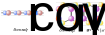
\includegraphics[width=0.5\linewidth]{img/fig-delta.pdf}
% \caption{\label{fig-delta} Scheme for the determination of the
  % covalent thickness of one-atom-thick (left) and few-atom-thick
  % (right) 2D materials.}
  % \end{figure}
\begin{table}[H]
  \centering
  \caption{In-plane ($r_{0}^{\parallel}$) and out-of-plane
    ($r_{0}^{\perp}$) radii of the polarizability ellipsoid of
    selected 2D materials calculated from first principles
    simulations. $r_{0}^{\parallel}$ is in general much larger than
    $r_{0}^{\perp}$, which accounts for the highly anisotropic
    dielectric nature of 2D materials.}
  \label{tbl:radii}  
  \begin{tabular}{lcc}
    \hline
    Material & $r_{0}^{\parallel} = \alpha_{\mathrm{2D}}^{\parallel}/2\varepsilon_{0}$ (\AA{}) &  $r_{0}^{\perp} = \alpha_{\mathrm{2D}}^{\perp}/2\varepsilon_{0}$ (\AA{})\\
    \hline
    2H-MoS$_{2}$ & 40.0 & 2.50 \\
    2H-MoSe$_{2}$ & &  \\
    2H-MoTe$_{2}$ & 58.1 & 3.07  \\
    2H-WS$_{2}$ & 35.7 & 2.46  \\
    2H-WSe$_{2}$ & 41.0 & 2.71 \\
    2H-WTe$_{2}$ & 53.5 &  3.17\\
    \hline
  \end{tabular}
\end{table}

\begin{figure}[H]
\centering
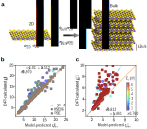
\includegraphics[width=0.75\linewidth]{./img/fig4.pdf}
\caption{\label{fig-4} \textbf{Transition of dielectric properties
    from 2D to 3D systems}. \textbf{a}. Scheme for the 2D-3D
  transition. $\alpha$ in the 2D material is essentially equivalent to
  $\varepsilon$ in its bulk counterpart. \textbf{b}
  $\varepsilon_{\mathrm{bulk}}^{\parallel}$ calculated from DFT
  (y-axis) compared with the predicted value from 2D
  $\alpha_{\mathrm{2D}}^{\parallel}$ (x-axis), showing good correlation. \textbf{c}
  $\varepsilon_{\mathrm{bulk}}^{\perp}$ calculated from DFT (y-axis)
  compared with the predicted value from 2D $\alpha_{\mathrm{2D}}^{\parallel}$
  (x-axis). The predicted value is in good aggreement with the DFT
  calculation when $E_{\mathrm{g}}>4$ eV, due to minimal interlayer
  coupling. The comparisons in \textbf{b} and \textbf{c} are made
  based on both HSE06 (circles) and PBE (squares) levels.}
\end{figure}

\begin{figure}[H]
  \centering
  \includegraphics[width=0.95\linewidth]{img/fig5.pdf}
  \caption{\textbf{Phase diagram of dielectric anisotropy $\eta$ as
      function of bandgap $E_{\mathrm{g}}$}. The
    $\eta$-$E_{\mathrm{g}}$ values of 2D materials (blue triangle) and
    their bulk counterparts (orange square) can be distinguished by
    the line $\eta=0.048(E_{\mathrm{g}}/\mathrm{eV})+0.087$. $\eta-E_{\mathrm{g}}$ values of
    semiconducting materials in other dimensions are also superimposed
    for comparison. Isotropic dielectric property is observed for bulk
    covalent materials (3D, red triangle) and fullerenes (0D, green
    star), while reduced dimensional materials, including planar
    organic semiconductor(OSc, 1D-2D, brown triangle), carbon nanotube
    (CNT, magenta circle) and linear OSc (0D-1D, violet pentagon) are
    scattered along the boundary line. The dimensionality and
    structure of typical materials are shown along the axis on the
    right. Compared with other materials, 2D materials and their bulk
    counterparts provide more flexibility of controlling the
    dielectric anisotropy.}
  \label{fig:aniso}
\end{figure}

\end{document}